\section{System Setup}\label{section:SystemSetup}

The system's performance has to be measured without influencing the program's run. This purpose serves the Node LVAnalyzer, which only subscribes to several topics and does not publish any messages. This node performs the complete performance analysis of the system.\par
This node contains a class Analyser, which performs the entire analysis. After the initialization, the class can be used by repeatedly calling its method insert. This method takes an id of a newly classified scene together with the robot's position and orientation at the scene's time. If the id is new, the position and orientation are stored, and all previously stored positions and orientations are compared to detect possible false negative. If the id already exists, the current position and orientation are compared with the stored one to detect possible false positive evaluation.\par
If the insert method is called on all scenes during the algorithm's run, the total number of true and false positives and a total number of true and false negatives is calculated. Furthermore, the analyzer generates detailed information, like ids, time, and exact positions of all false positive and negative evaluations. In addition to that, if the scene images are passed as a third optional parameter to the insert method, the Analyser will generate images of all false positive evaluations to see the difference between the wrongly matched views. This class also provides an animated live preview of all the scenes and their matches, as shown in Figure \ref{fig:analExample}.\par

\begin{figure}[htpb]
    \centering
    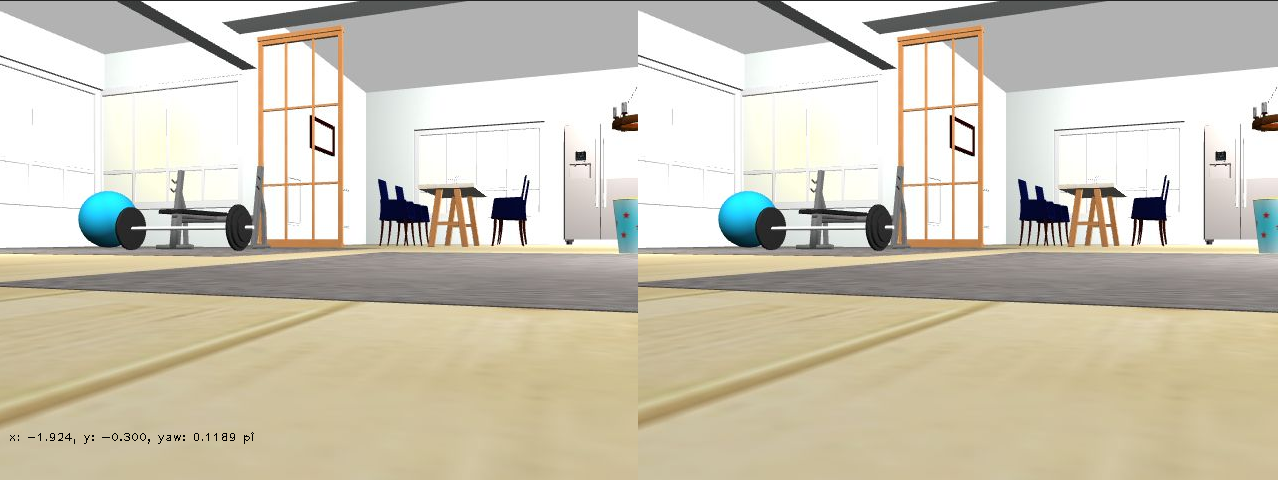
\includegraphics[width=0.8\textwidth]{analyserExample.png}
    \caption[Preview of the animation generated by the analyzer]{Preview of the animation generated by the analyzer. The left part shows a current scene and position, and the right part shows the preview of a matched scene.} \label{fig:analExample}
\end{figure}

The LVAnalyzer node is a wrapper over the Analyser class. This node subscribes to three topics, LVTemplate, Odometry, and Camera. After receiving a new matched template id from the LVTemplate topic, the exact position and scene image is found from the Odometry and Camera topics based on the timestamp of the messages. Afterward, all information is passed to the Analyser class using the insert method.
